\problemname{}

\illustration{0.2}{fish.png}{
    CC BY-SA 4.0 by ChatGPT
}


Vous êtes un explorateur marin, vous avez fait une découverte dans les profondeurs de l'océan, là où la lumière du soleil ne peut plus atteindre, une étrange espèce de poisson bioluminescent, connue sous le nom de Karwa.

Ces poissons ont une particularité assez spéciale : ils ont des écailles réfléchissantes qui réfléchissent la lumière dans des directions précises.

Vous décidez donc d'en apprendre un peu plus sur cette espèce de poisson, plus particulièrement leurs positions. En effet, il semblerait qu'il y ait un certain pattern dans leurs positions.

Pour ce faire, vous avez enregistré la position de tous les karwas aux alentours, mais le problème est qu'il y a plusieurs bandes de karwas au même endroit. Votre but est de déterminer combien de karwas font partie d'une bande étant donné un poisson spécifique.

Vous avez remarqué que 2 karwas font partie de la même bande si en envoyant de la lumière sur un des karwa, la lumière est réfléchie sur l'autre karwa.

Heureusement, vous avez aussi enregistré dans quelle direction chaque karwa réfléchit la lumière. Cette direction est exprimée en degrés et étonnamment, c'est toujours un nombre entier.

\smallskip
\begin{figure}[h]
    \centering
    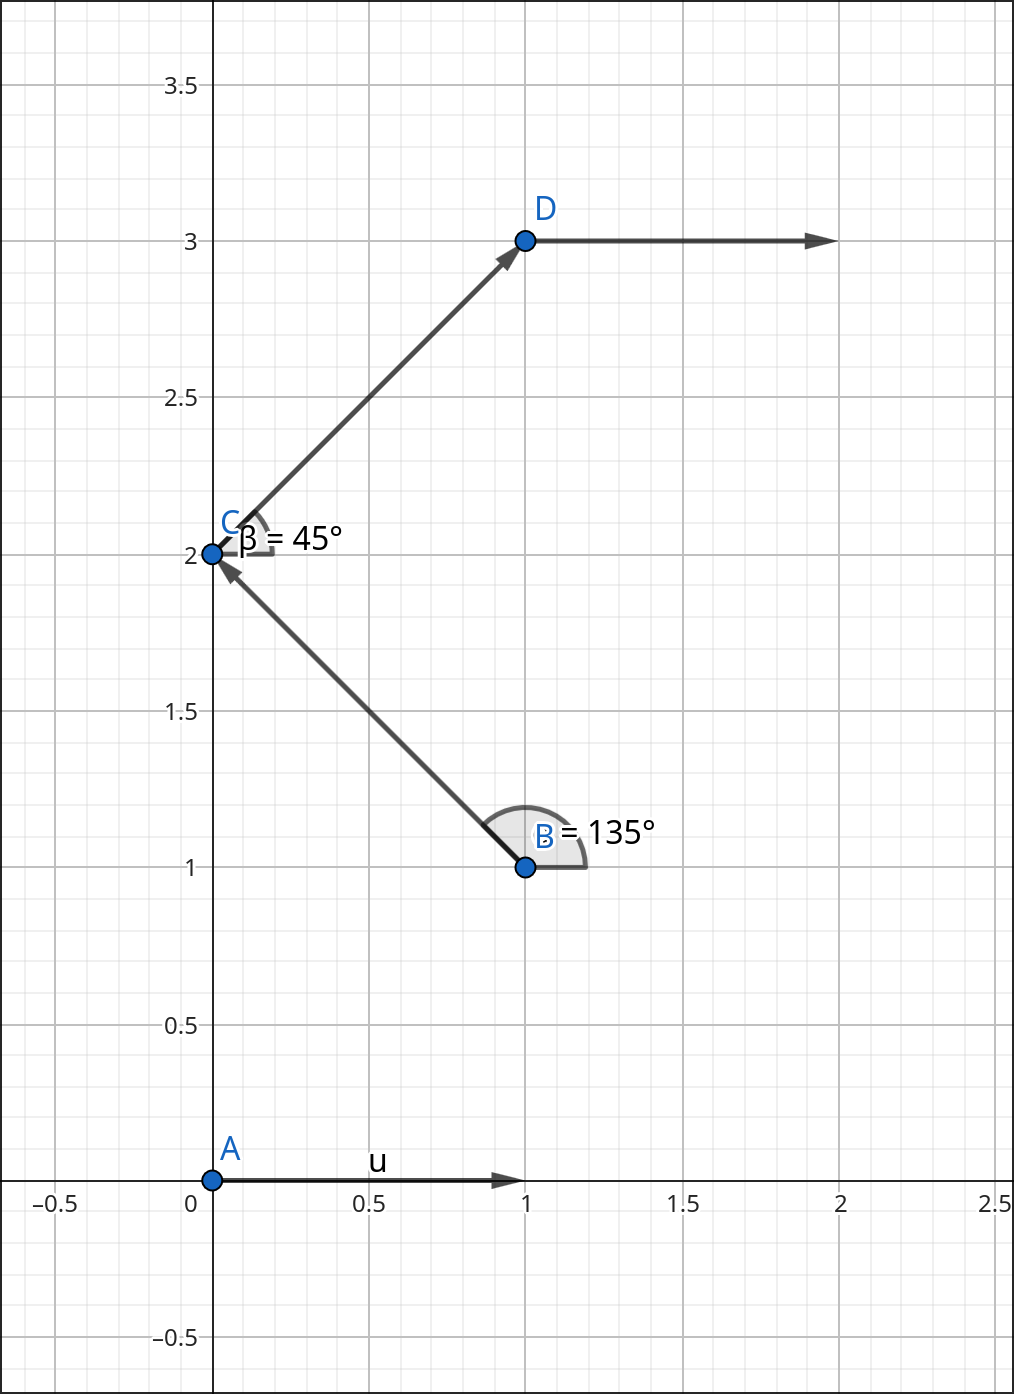
\includegraphics[width=0.3\textwidth]{sample1.png}
    \caption{Exemple du sample 1}
\end{figure}

\begin{Input}
    L'entrée consiste en :
    \begin{itemize}
        \item Une ligne avec un entier $n$ ($1 \leq n \leq 10^{5}$), le nombre de poissons.
        \item $n$ lignes avec deux nombres RÉELS $x, y$ ($-10^{18} \leq x,y \leq {10^{18}}$) et un entier d, ($0 \leq d < 360$). Qui sont respectivement l'emplacement du poisson ainsi que la direction dans laquelle ils réfléchissent la lumière.
        \item Une ligne avec un entier $a$ ($0 \leq a < n$) qui est le poisson que vous analysez.
    \end{itemize}
\end{Input}

\begin{Output}
    La taille de la bande.
\end{Output}
